\documentclass[parskip=full]{scrartcl}
\usepackage[T1]{fontenc}    % avoid garbled Unicode text in pdf
\usepackage[utf8]{inputenc} % use utf8 file encoding for TeX sources
\usepackage[german]{babel}  % german hyphenation, quotes, etc
\usepackage{hyperref}       % detailed hyperlink/pdf configuration
\hypersetup{                % ‘texdoc hyperref‘ for options
pdftitle={PSE: Entwicklung eines relationalen Debuggers - Pflichtenheft},%
,%
}
\usepackage{graphicx}       % provides commands for including figures
\usepackage{csquotes}       % provides \enquote{} macro for "quotes"
\usepackage[nonumberlist]{glossaries}     % provides glossary commands
\usepackage{enumitem}
\usepackage{xcolor}
\newcommand\frage[1]{\textcolor{red}{#1}}


\font\myfont=cmr12 at 20pt

\title{
	\vspace{2cm}
	\myfont 
	Praxis der Softwareentwicklung:\\ 
	Entwicklung eines relationalen Debuggers\\
}
\subtitle{
	\vspace{1cm}
	\myfont
	Entwurfsdokument
}
\author{
	\vspace{1cm} \\
	Benedikt Wagner\\
	\texttt{udpto@student.kit.edu}
	\and \vspace{1cm} \\ Chiara Staudenmaier\\
	\texttt{uzhtd@student.kit.edu}
	\and Etienne Brunner\\
	\texttt{urmlp@student.kit.edu}
	\and Joana Plewnia\\
	\texttt{uhfpm@student.kit.edu} 
	\and Pascal Zwick\\
	\texttt{uyqpk@student.kit.edu}
	\and Ulla Scheler\\
	\texttt{ujuhe@student.kit.edu}
	\vspace{1cm}
	\and Betreuer: Mihai Herda, Michael Kirsten
	\vspace{4cm}
}


\begin{document}
\clearpage
\maketitle
\pagenumbering{gobble}
\newpage

\tableofcontents
\newpage
\pagenumbering{arabic}
%Eventuell Fußnoten generieren
\section{Einleitung}
%Einleitung mit grobem Überblick. Dieser Abschnitt soll an das Pflichtenheft anschließen.
Dieses Dokument dokumentiert den Entwurf des Produkts \enquote{DIbugger}, wie es im Pflichtenheft definiert wurde.\\
Hierbei werden das Geheimnisprinzip und Lose Kopplung berücksichtigt, um für erhöhte Verständlichkeit
zu sorgen.
\section{Paketeinteilung} %eventuell fällt jemandem ein besserer Titel ein
%Paketdiagramm, Erläuterung der Einteilungsentscheidung, Schnittstellen
\subsection{Übersicht}

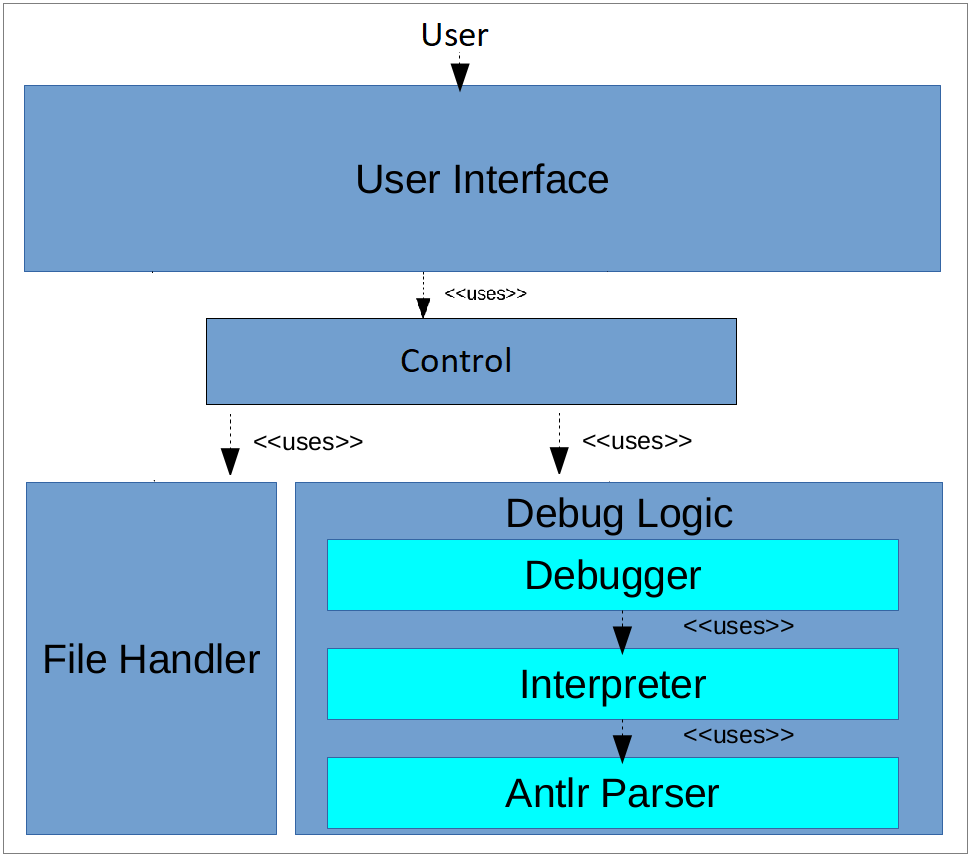
\includegraphics[scale=0.35]{../Plichtenheft/Architektur.png} \\
Das Produkt ist aufgeteilt in die Pakete \enquote{Control}, \enquote{User Interface}, \enquote{File Handler} und \enquote{Debug Logic}.
Hierbei besteht die Debug Logic aus den Unterpaketen \enquote{Debugger}, \enquote{Interpreter} und
\enquote{Antlr Parser}.


\subsection{User Interface}
\paragraph{Aufgaben} Das Paket User Interface stellt die Möglichkeit zur Kommunikation des Nutzers mit dem Produkt dar. Hierbei dient dieses Paket als View Teil des MVC-Konzepts.
\paragraph{Schnittstellen} 
\begin{itemize}
\item Angebotene Schnittstellen:\\
Es wird eine Fassade angeboten, welche es ermöglicht Variablen, Programmtexte und Eingaben anzuzeigen.
\item Genutzte Schnittstellen:\\
Dieses Paket nutzt die Control-Fassade und deren angebotenen Schnittstellen.
\end{itemize}
\paragraph{Benutztrelation} Das Paket User Interface benutzt die Control-Fassade um an jegliche, durch den Benutzer angeforderte, Information zu gelangen, bzw. das vom Benutzer geforderte auszuführen. Da das Paket User Interface die oberste Schicht des Schichtendiagramms darstellt, wird dieses von keinen anderen Paketen benutzt. 


\subsection{Control}
\paragraph{Aufgaben}
\paragraph{Schnittstellen}
\paragraph{Benutztrelation}

\subsection{File Handler}
\paragraph{Aufgaben}
Das Paket FileHandler stellt die Funktionalität zum Lesen, Schreiben, Parsen und Interpretieren von sämtlichen Dateien bereit und siedelt sich im Model Teil des MVS-Konzepts an.
Dabei wandelt dieser eine Konfigurationsdatei, welche auf dem Dateisystem gespeichert ist, in eine virtuelle Datei um.
Diese besteht aus einer Klassenstruktur, welche äquivalent zur Definition des Speicherformats ist, also Zuweisungen und Blöcke.
Weiter erzeugt der FileHandler Objekte der Konfigurations-, Sprach- und Einstellungsdateien und kann diese nach außen weitergeben.
\paragraph{Schnittstellen}
\begin{itemize}
\item Genutzte Schnittstellen: \\
Der FileHandler benötigt keine Schnittstellen anderer Programmpakete, da er an unterster Stelle in der Benutztrelation steht.
\item Angebotene Schnittstellen: \\
Es werden eine Fassade und drei Klassen angeboten.
Diese repräsentieren die Dateien für Produkteinstellungen, Sprachen (Übersetzungen der GUI) und Laufkonfigurationen.

\end{itemize}
\paragraph{Benutztrelation}
Der FileHandler hat keine Unterpakete und steht an unterster Stelle der Benutztrelation.
Somit entstehen auch keine Abhängigkeiten zu anderen Paketen.

\subsection{Debug Logic}
Das Paket \textit{DebugLogic} stellt den Model Teil der MVC Architektur dar. Die interne Struktur des Paketes ist eine intransparente 3-Schichten-Architektur.\\
Die unterste Schicht stellt das Subpaket \textit{DebugLogic.AntlrParser} dar. Es erzeugt aus einfachen Zeichenketten Ableitungsbäume nach den Ableitungsregeln der in \ref{FormSpez} gegebenen Grammatiken.\\ Darauf aufbauend in der mittleren Schicht finden sich die Subpakete \textit{DebugLogic.TraceGenerator} und \textit{DebugLogic.RelationalExpressionGenerator}, die beide die Aufgabe haben, diese Ableitungsbäume durch interpretieren in eine abstrakte und leicht handhabbare Form zu bringen. Da beide Subpakete eine gemeinsame Schicht darstellen, findet hier auch ein hohes Maß an Kommunikation statt. \\ In der obersten Schicht ist das Subpaket \textit{DebugLogic.Debugger} angesiedelt. Dieses nutzt die abstrakten Repräsentationen und führt den eigentlichen Debugprozess darauf aus.
\subsubsection{Debugger}
\subparagraph{Aufgaben}
Der Debugger nutzt die von den Subpaketen \textit{DebugLogic.TraceGenerator} und \textit{DebugLogic.RelationalExpressionGenerator} erzeugten Informationen, um Watch-Expressions und bedingte Breakpoints auszuwerten, sowie die üblichen Debugmechanismen zu steuern.
\subparagraph{Schnittstellen}
Als oberste Schicht des Paketes \textit{DebugLogic} stellt dieses Subpaket die gleichen Schnittstellen wie die DebugLogic bereit.
\subparagraph{Benutztrelation} 
Das Subpaket benutzt die Subpakete \textit{DebugLogic.TraceGenerator} und \textit{DebugLogic.RelationalExpressionGenerator}.
Um die üblichen Debugmechanismen wie Schritte und Weiter durchführen zu können, nutzt dieses Subpaket den vom Subpaket \textit{DebugLogic.TraceGenerator} bereitgestellten Iterator. 
Um WatchExpressions und bedingte Breakpoints auszuwerten und zu repräsentieren, nutzt dieses Subpaket die vom Subpaket \textit{DebugLogic.RelationalExpressionGenerator} bereitgestellte abstrakte Repräsentationen.
\subsubsection{Trace Generator}
\subparagraph{Aufgaben}
Dieses Subpaket nimmt den Quelltext eines WLang-Programms entgegen und hat die Aufgabe, einen Pfad über den gesamten Programmfluss dessen zu erzeugen, sodass später darüber iteriert werden kann. Dazu gehört auch das Prüfen auf semantische Fehler, etwa das Fehlen eines return Statements.
\subparagraph{Schnittstellen}
\begin{itemize}
\item Angebotene Funktionalität:\\
Stellt einen Iterator über den Ausführungspfad eines gegebenen Programmes zur Verfügung.
\item Genutzte Funktionalität:\\
Nutzt Syntax-Prüfung und Syntaxbaum-Erzeugung des Subpakets \textit{DebugLogic.AntlrParser}. 
\end{itemize}

%TODO Schnittstellen in Form von Facade
\subparagraph{Benutztrelation} 
Das Unterpaket benutzt das Unterpaket \textit{DebugLogic.AntlerParser}, um damit aus den reinen Zeichenketten einen Syntaxbaum gemäß der in \ref{FormSpez} gegebenen Grammatik für die Sprache WLang erzeugen zu lassen. Auf dieser Vorraussetzung baut die Arbeit des Subpakets auf.
\subsubsection{Relational Expression Generator}
\subparagraph{Aufgaben}
Dieses Subpaket nimmt Zeichenketten, die Watch-Expressions und bedingte Breakpoints beschreiben, entgegen und hat die Aufgabe, diese zu interpretieren. Dazu wird in diesem Paket eine abstrakte Darstellung dieser erzeugt.
\subparagraph{Schnittstellen}
\begin{itemize}
\item Angebotene Funktionalität:\\
Erzeugt aus gegebenen Zeichenketten für Watch-Expressions und bedingte Breakpoints eine abstrakte Repräsentation, sodass diese dann leicht ausgewertet werden kann.
\item Genutzte Funktionalität:\\
Nutzt Syntax-Prüfung und Syntaxbaum-Erzeugung des Subpakets \textit{DebugLogic.AntlrParser}. 
\end{itemize}
%TODO Schnittstellen in Form von Facade
\subparagraph{Benutztrelation} 
Das Unterpaket benutzt das Unterpaket \textit{DebugLogic.AntlerParser}, um damit aus den reinen Zeichenketten einen Syntaxbaum gemäß der in \ref{FormSpez} gegebenen Grammatik für Watch-Expressions und Bedingte Breakpoints erzeugen zu lassen. Auf dieser Vorraussetzung baut die Arbeit des Subpakets auf.
\subsubsection{Antlr Parser}
\subparagraph{Aufgaben}
\subparagraph{Schnittstellen}
\subparagraph{Benutztrelation} 

\section{Beschreibung der Klassen}
Detaillierte Beschreibung aller Klassen. Das beinhaltet (JavaDoc) Beschreibungen zu allen Me-
thoden, Konstruktoren, Packages und Klassen. Was hier nicht reingehört sind private Felder
und Methoden. Das sind Implementierungsdetails.

\subsection{Klassen in Paket 1}
\subsection{Klassen in Paket 2} 
...

\section{Charakteristische Abläufe}
Beschreibung von charakteristischen Abläufen anhand von Sequenzdiagrammen. Beispielswei-
se bieten sich Testszenarien aus dem Pflichtenheft hier an. Wir empfehlen Sequenzdiagramme
möglichst früh zu erstellen, denn dabei werden die Schnittstellen zwischen Packages und Klas-
sen klar. 
Auf Klassen oder Pakete in Beschreibung aller Klassen verweisen


\section{Abhängigkeitseinteilung}
Mit Blick auf den Implementierungsplan: Aufteilung in Klassen/Pakete, die unabhängig vonein-
ander implementiert und getestet werden können.

\section{Formale Spezifikation von Kernkomponenten}\label{FormSpez}
Speicherformate, Sprachdefinition(formal)

\section{Änderung zum Pflichtenheft}
Änderungen zum Pflichtenheft, z.B. gekürzte Wunschkriterien.




\section{Anhang}
UML-Klassendiagramm 
Vollständiges großformatiges Klassendiagramm im Anhang. Ausschnitte/Teile können bereits
vorher verwendet werden, um Teilkomponenten zu beschreiben. Assoziationen zwischen Klas-
sen dabei bitte mit entsprechenden Pfeilen darstellen, statt nur durch Feldtypen.
Identifikation von Entwurfsmustern um Struktur gröber zu beschreiben.





\end{document}
\grid
